\def\year{2019}\relax
%File: formatting-instruction.tex
\documentclass[letterpaper]{article} %DO NOT CHANGE THIS
\usepackage{aaai19}  %Required
\usepackage{times}  %Required
\usepackage{helvet}  %Required
\usepackage{courier}  %Required
\usepackage{url}  %Required
\usepackage{graphicx}  %Required
\frenchspacing  %Required
\setlength{\pdfpagewidth}{8.5in}  %Required
\setlength{\pdfpageheight}{11in}  %Required
%PDF Info Is Required:
  \pdfinfo{
/Title (Title and Image Based Classification of Magic: The Gathering Cards)
/Author (Derick Anderson, Zachary Reiter)}
\setcounter{secnumdepth}{0}  
\nocopyright
\graphicspath{ {./imgs/} }
 \begin{document}
% The file aaai.sty is the style file for AAAI Press 
% proceedings, working notes, and technical reports.
%
\title{Title and Image Based Classification of Magic: The Gathering Cards}
\author{Derick Anderson \ and Zachary Reiter\\
  anderson.derick.w@gmail.com\\
  reiter.z@husky.neu.edu
}
\maketitle
\begin{abstract}
magic!
\end{abstract}



\section{Background}

is a card game

\section{Project Description}



\subsection{Title-based Classification}

The architecture used for title classification
was a character-level LSTM with self-attention.
The LSTM \cite{Hochreiter1997LongSM} is a recurrent neural network architecture
that is frequently and effectively \cite{Schmidhuber2015DeepLI}
used to process text data.
Because it is such a well known architecture
we will not reproduce here its fundamental structure.
We will discuss the extensions to the basic LSTM that were used.

The LSTM was character-level,
which means that timesteps were taken to be each character in the title.
The characters were embedded in vector space
before being passed into the LSTM as input.
The character embeddings were learned from scratch
in a fully end-to-end manner.

Attention is a mechanism for combining a sequence of values into a single value
with learnable parameters.
We use the multi-headed self-attention mechanism from \cite{Lin2017ASS}
over the outputs of the LSTM and before our output layer.
It was shown to enhance peformance on some classification tasks
(as compared to passing the final state of the LSTM to the output layer)
and as a bonus permits attractive visualizations
of which portions of the input sequence contribute to the output.

The optimizer used was Adam \cite{Kingma2014AdamAM}
with norm-based gradient clipping \cite{Pascanu2012UnderstandingTE}.

\begin{figure}
  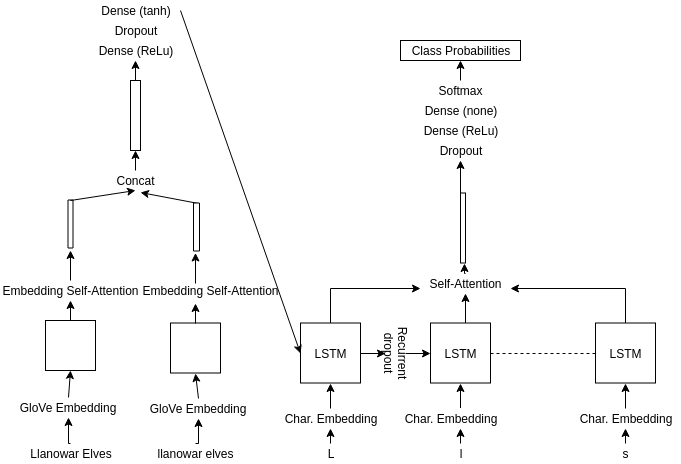
\includegraphics[width=.5\textwidth]{text-architecture}
  \caption{Title-based model architecture}
\end{figure}

\subsubsection{Word Embeddings}

In one variation of the model
the initial state of the LSTM
is created from the embeddings of words in the title.
We used pre-trained GloVe \cite{Pennington2014GloveGV} embeddings,
specifically the 840B token Common Crawl set
available for download from the Stanford NLP group's website
\footnote{https://nlp.stanford.edu/projects/glove/}.
Using pre-trained word embeddings
was motivated by the need for lexical knowledge in classifying titles.
On an intuitive level many titles for creatures
contain words that describe people/animals etc,
and the other categories likewise often have informative English words.

We combine sequences of word embeddings with a small self-attention layer.
That set of word embeddings is case-sensitive,
so we concatenate the attended result of embedding
the word-level tokens of the title as-is
and the tokens converted to lower case.
Card titles are title cased,
so it was helpful to get the embedding of common nouns in the title
in their lower cased form.
For example,
``Merfolk Looter''
has a more informative (and more likely to be in the vocabulary)
embedding for ``looter'' than for ``Looter''.

The GloVe data we downloaded has a vocabulary of over 2 million ``words'',
but we use only the embeddings representing the most common 200,000.
On a practical computational level,
it is difficult to incorporate such large matrices into a model.
On another level,
it was observed that many MtG-specific proper nouns are in the full vocabulary.
Insofar as Magic: The Gathering is a popular topic online and the word embeddings
are based on web crawl data that only makes sense.
However,
it was considered not quite in the spirit of the task
for MtG-specific proper nouns to be in-vocabulary.
A selection of the most common MtG-specific proper nouns were investigated
and found to be below the 200,000th most common mark.
More general myth-related or fantastical terms (e.g. ``elf'', ``merfolk'')
largely remained in the vocabulary.
Out-of-vocabulary terms were assigned a randomly initialized embedding.

\subsubsection{Regularization}

Given the small size of the training data thorough regularization was a must.
The methods of regularization used were
L2 regularization on the weights of the dense layers,
dropout between dense layers,
recurrent dropout (as described in \cite{Gal2016ATG}) in the LSTM,
and the penalty described in \cite{Lin2017ASS} for the self-attention layer.
Card titles consisted only of ASCII characters;
the distribution of characters was not particularly sparse
and so no regularization directly on the character embeddings
was thought to be necessary.
No regularization was needed on the word embeddings since they were not trained.

\section{Experiments}


\subsection{Title-based Classification}

\begin{table}
  \centering
  \caption{Hyperparameters of the final title-based model}
  \begin{tabular}{r | c | c}
    Hyperparameter & Value (small) & (large) \\
    \hline
    LSTM Size & 256 & 512 \\
    Character embedding size & 64 & 128 \\
    Attention, number of heads ($r$) & 3 & 3\\
    Attention, attention size ($d_a$) & 64 & 128\\
    Dropout rate & 0.5 & 0.5 \\
    L2 regularization coef. & 1e-4 & 1e-4 \\
    Attention regularization coef. & 4e-4 & 4e-4 \\
    Gradient clipping threshold & 5.0 & 5.0 \\
  \end{tabular}
\end{table}

Unfortunately,
due to time constraints,
there was not the opportunity for an organized hyperparameter search.
Instead,
reasonable values were chosen from experience and the literature
and only a little local search performed.
Interestingly the smaller configuration outperformed the larger configuration
on the reported results.
That can be attributed partially to noise in the results,
and also to the danger of overfitting on the small data.
Either way,
the smaller model configuration is therefore used for all following analyses.
It is clear from the results that the lexical knowledge supplied by word vectors
is very helpful to the model.

\begin{table}
  \centering
  \caption{Test scores on all data for different model configurations}
  \begin{tabular}{r | c | c}
    Model configuration & Accuracy & Macro-averaged F1 \\
    \hline
    Small & 80.6\% &  .642 \\
    Larger & 79.2\% & .638 \\
    Character-only & 71.3\% & .523 \\
    Largest class & 55.6\% & .179 \\
  \end{tabular}
\end{table}

It is interesting to compare the speed with which the character-only
and the full model learned.
The full model reached its maximum accuracy on the validation set quite quickly,
whereas it took the character-only model 25 epochs to reach its maximum.
That the character model can productively learn for 25 epochs
suggests that either the character information is redundant
in the presence of word embeddings
or the full model isn't learning optimally.
Looking at the distribution of attention intensity
also suggests that the full model doesn't pay a lot of attention to the characters.
The attention heads for the character model focus at a few different points,
the embedding model's attention is much more diffuse
(except for at the first position,
where I speculate the first head reports
the information gained from the initial state).

\begin{figure}
  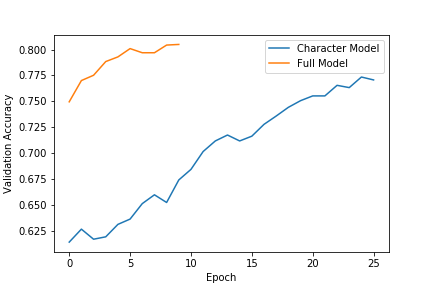
\includegraphics[width=.5\textwidth]{training-speed-comparison}
  \caption{Validation accuracy over time for character-only model vs. full model}
\end{figure}

\begin{figure}
  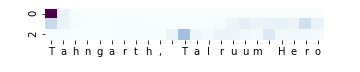
\includegraphics[width=.5\textwidth]{tahngarth-attention-wv}
  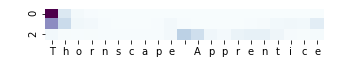
\includegraphics[width=.5\textwidth]{thornscape-attention-wv}
  \caption{Attention intensity for full model}
\end{figure}

\begin{figure}
  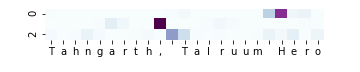
\includegraphics[width=.5\textwidth]{tahngarth-attention-char}
  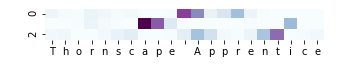
\includegraphics[width=.5\textwidth]{thornscape-attention-char}
  \caption{Attention intensity for character-only model}
\end{figure}

\begin{table}
  \centering
  \caption{Macro-averaged F1 by training and testing dataset}
  \begin{tabular}{r | c | c | c}
    & \multicolumn{3}{c}{Test dataset}\\
    \cline{2-4}
    Train dataset & all & modern & legacy \\
    \hline
    all    & .642 & .643 & .645 \\
    modern & .602 & .643 & .573 \\
    legacy & .622 & .597 & .639 \\
  \end{tabular}
\end{table}

\begin{table}
  \centering
  \caption{Accuracy by training and testing dataset}
  \begin{tabular}{r | c | c | c}
    & \multicolumn{3}{c}{Test dataset}\\
    \cline{2-4}
    Train dataset & all & modern & legacy \\
    \hline
    all    & 80.6\% & 81.2\% & 80.1\% \\
    modern & 76.0\% & 78.3\% & 74.1\% \\
    legacy & 76.4\% & 75.1\% & 77.0\% \\
  \end{tabular}
\end{table}

As predicted from the beginning,
training on one of the genres of data
and testing on the other genre leads to reduced performance.
It appears that training on the legacy cards
transfers more easily to the modern cards
than vice-versa,
to the tune of a few points of accuracy.

\begin{figure}
  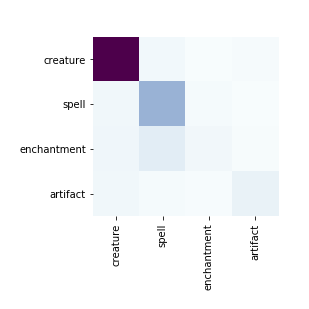
\includegraphics[width=.5\textwidth]{text-confusion-matrix}
  \caption{Confusion matrix: predicted is on the x axis}
\end{figure}

The confusion matrix matches our intuitions fairly well.
The two classes with the largest confusion are spell and enchantment,
which while distinct in the game mechanics
are certainly the semantically closest in an abstract sense.

\bibliography{doc}
\bibliographystyle{aaai}

\end{document}


%%% Local Variables:
%%% mode: latex
%%% TeX-master: t
%%% End:
